High-performance computing (HPC)是指使用超级计算机或者计算机集群来解决需要大量计算的复杂计算问题,
通常需要集成多个处理器构成一个计算机系统,并且还需要协同进行分布式计算和并行计算。\cite{wiki_hpc}

借助于HPC,可以将原本需要计算数年的任务缩短到几天甚至更短,
对于HPC而言,最关键的指标就是其算力究竟有多强。
衡量算力通常使用\textit{每秒浮点运算次数( floating point operations per second)}\cite{wiki_flops}来表示,
其单位为$FLOP/s$。
在具体计算时,又可以分为两种方式:
\begin{itemize}
    \item \textbf{计算理论最大性能(peak)}:通过计算时钟频率乘以单个时钟周期完成双精度浮点数操作次数得出,如$2.5\;Ghz \times 4\;FLOP/clock = 10 \;GFLOP/s$,但是受限于I/O操作等,实际不可能达到
    \item \textbf{计算真实性能(real)}:通过一些程序进行持续计算并得出观测结果,例如\href{https://www.top500.org/}{Top500}使用\href{https://netlib.org/linpack/}{Linpack}进行线性代数运算。
\end{itemize}

2019年超算就可以执行超过千万亿次 FLOPS。
相比之下,高端游戏台式机的速度要慢 1,000,000 倍以上,
可执行约 200 千兆次 FLOPS (1 × 109)\cite{amd_hpc}。

\subsection{HPC的应用领域}
HPC最早是应用在数学和物理学领域,如今HPC的应用范围已经非常广泛,
主要围绕在一些超算问题解决上面\cite{hpc_book}:

\begin{itemize}
    \item \textbf{偏微分方程求解}: 包括物理、工业上的一些方程求解,
    如麦克斯韦方程、Black-Scholes方程等,以及流体力学研究、天气预报等
    \item \textbf{线性代数}: 包括搜索引擎PageRank、有限元模拟、线性代数建模等
    \item \textbf{两两耦合相互作用的大型系统}:包括宇宙学、分子动力学模拟等
    \item \textbf{图问题}: 包括机器学习、欺诈识别、数据分析等
    \item \textbf{随机系统}: 包括粒子物理学研究、核反应堆设计、模拟疾病传播等
\end{itemize}

抛开具体的领域,单从问题本身对于算力、存储等的要求来看,
HPC可以解决的问题可以归纳为以下几类\cite{hpc_problem_types}:

\begin{itemize}
    \item \textbf{计算密集型}: 解决问题需要进行大量的计算工作,
    譬如进行金融建模、风险敞口等,
    这类问题是传统HPC应用最多的类别
    \item \textbf{内存密集型}: 解决问题需要使用大量的内存,
    相对于计算密集型问题,这类问题对内存的大小、不同节点内存的性能差异
    以及CPU、内存的交互上更敏感
    \item \textbf{数据密集型}: 解决问题时需要处理大的数据集,
    即“大数据”问题
    \item \textbf{高吞吐量型}: 需要批量计算大量的无关任务,
    例如大量的任务运行,彼此间无需CPU级别通信,
    在单独的线程上并行运行。
    例如,一家企业可能向某节点集群中的各个处理器核心提交了 1 亿条信用卡记录\cite{oracle_hpc}。
\end{itemize}

除了传统的超算问题外,
一些新兴的领域也在探索与HPC进行融合,
成为HPC的重要应用场景,包括:
\begin{itemize}
    \item \textbf{高性能数据分析(HPDA)}: 为了支持日益复杂的算法,
    高性能数据分析(HPDA)已成为一个将 HPC 资源应用于大数据的新细分领域。
    包含统计分析、数据清洗、数据汇聚等,
    借助HPDA可以将大数据处理系统(如Hadoop、Spark)等与HPC融合起来,
    一方面实现全流程的加速处理,
    另一方面大数据也可以与HPC的技术相互受益\cite{hpda,yef2022_hpc}
    \item \textbf{人工智能(AI/ML/DL)}: 包含三大类应用,
    一类是以卷积网络为核心的图像检测、视频检索类问题,如安防、自动驾驶等;
    一类是以强化学习为核心的博弈决策类问题,如交通规划;
    一类是以Transformer为核心的自然语言处理类问题,如搜索推荐、智能人机接口等\cite{yef2022_hpc}
    \item \textbf{高级建模和模拟}: 高性能计算建模和模拟可用于药物研制和测试,
    汽车和航空航天设计、气候/天气系统预测以及能源应用\cite{amd_hpc}。
\end{itemize}

一份研究预测HPDA的市场增长从2018年到2023年为15.4\%,
超过全球HPC整体市场的预测增长7.8\%,
而HPC AI预测增长为29.5\%,远超HPDA\cite{hpc_rearch_2019}。

\subsection{HPC发展历史}

HPC的发展大致经过了以下几个阶段\cite{hpc_history}:

\begin{itemize}
    \item \textbf{1940s-1960s}: 诞生首个超级计算机。二次世界大战以及冷战催生了超级计算机的出现,来完成密码破译,以及核武器、飞机、潜艇设计等
    \item \textbf{1975-1990}: Seymour Cray(被誉为超级计算机之父)成立公司并发展了一系列超级计算机,如Cray-1 \textasciitilde 4
    \item \textbf{1990-2010}: 由单机转为集群以便能够利用更多的内存和CPU
    \item \textbf{2000-至今}: 进入混合加速的集群时代,由多核CPU、GPU加速节点等组成混合集群,对特定计算进行优化
\end{itemize}

\begin{figure}[ht!]
    \centering
    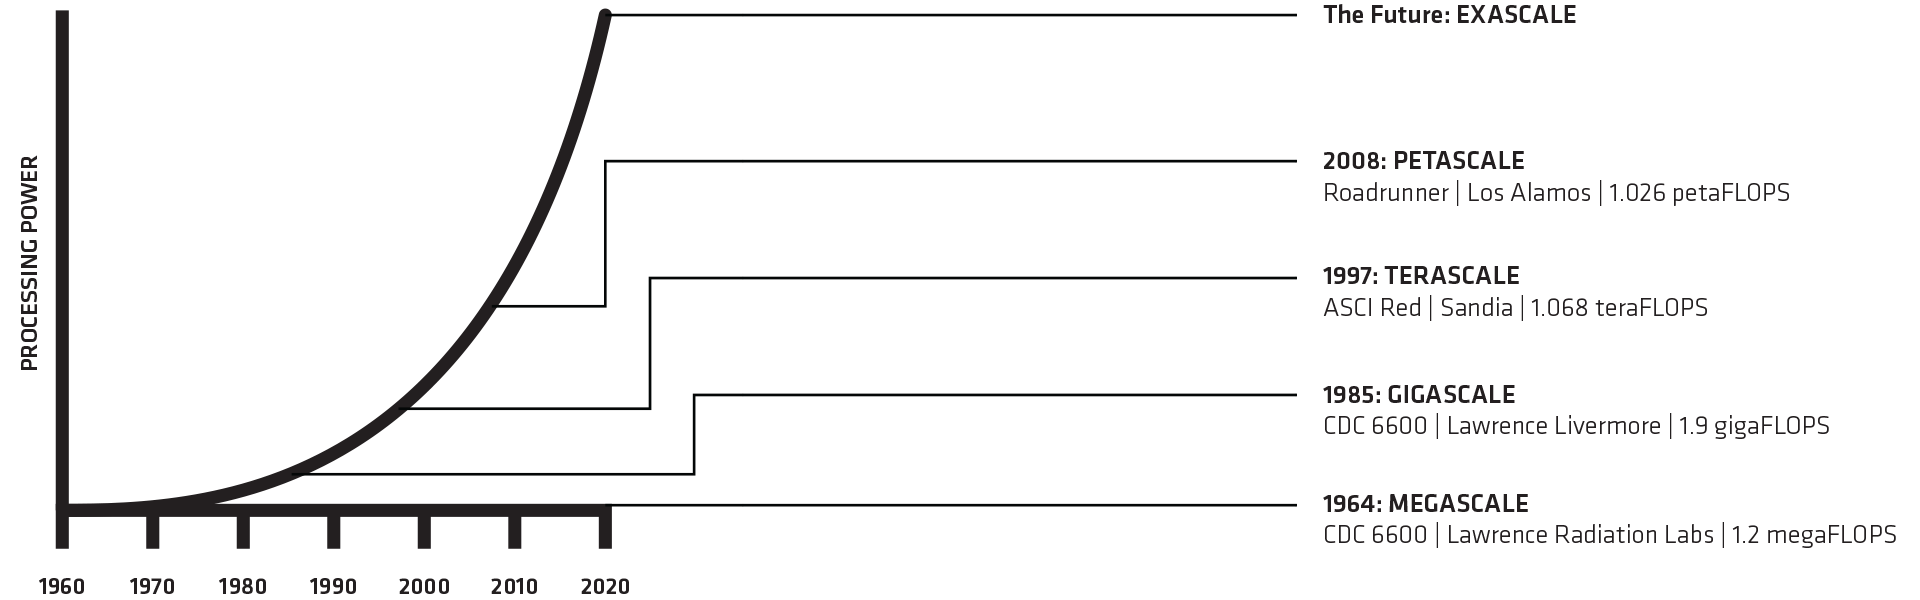
\includegraphics[width=\linewidth]{images/evolution-processing-power.png}
    \caption{世界HPC算力的变革}
\end{figure}
截至2022年9月,Top500上排名第一的超级计算机为Frontier(美国),其计算速度已达到$1.102 \;ExaFLOP/s$。

我国在过去十年依托顶尖的超算系统,大规模并行应用设计和研制方面取得显著进步,
多个超算应用入围戈登贝尔奖(ACM Gordon Bell Prize)
\footnote{戈登贝尔奖是国际高性能计算应用领域最高奖,设立于1987年,主要颁发给高性能应用领域最杰出成就。}
包括:
\begin{table}[ht]
\begin{tabularx}{\textwidth}{|p{3cm}|X|}
\toprule
\textbf{年份} & \textbf{应用} \\
\midrule
2014 & 地震模拟 \\
\hline
2016 &  大气动力框架、相场模拟、海浪模拟 \\
\hline
2017 &  地震模拟、大气模拟 \\
\hline
2018 &  图计算框架 \\
\hline
2021 &  量子模拟、人造太阳、第一性原理 \\
\bottomrule
\end{tabularx}
\end{table}

\subsection{HPC发展趋势}
传统的HPC计算以超算为代表,
超级计算机代表着高性能计算系统最尖端的水平。
由各个超算中心或者实验室开发,
尽管我国的超算能力处于世界领先水平,
但也存在着一系列的问题\cite{yef2022_hpc}:

\begin{itemize}
    \item 国产超算平台架构多样,应用移植和调优工作量大,
    例如神威·太湖之光(10,649,600 核,异构众核处理器SW26010,OpenACC*,Athread + MPI)与
    天河2号(498万核,2xCPU+2xMatrix2000,OpenMP,OpenCL+MPI)架构就不一样,
    程序在不同的超算系统间进行移植十分困难,而国外超算架构逐渐收缩到加速器异构,
    几乎是Intel CPU + NVIDIA GPU
    \item 对支持复杂应用全流程计算的能力不足
    \item 受制于美国定向打击制裁
\end{itemize}

随着云计算的成熟,
云平台强大的计算资源也成为了HPC的新基建。
除了超算中心外,民用和商用HPC也有着较大的发展,
包括微软、戴尔、Intel、IBM、AWS等均在HPC占有较大的市场份额。
国内有并行科技、阿里云、华为云、腾讯云等均有开放HPC业务。

近年来HPC发展有如下的趋势:

\begin{itemize}
    \item \textbf{异构高性能计算}: 将CPU 和GPU 等不同类型的计算单元结合在一起,
    被称为异构计算。常见的计算异构单元类别包括CPU、GPU、ASIC、FPGA等。 
    \item \textbf{向云上迁移}: HPC正朝向云端发展,一方面是因为问题复杂度越来越超出本地HPC的算力; 
    一方面,云计算允许按需提供资源,在成本和弹性上更有优势(公共云);
    一方面,在 HPC 中采用容器技术的势头也愈发显著\cite{redhat_hpc,oracle_hpc}。 
    调查显式,2019年已有超过10\%的HPC任务运行在云上,
    除了公有云外,私有云、混合云也在快速发展\cite{hpc_rearch_2019}。
    \item \textbf{与大数据融合}: HPC 有望与大数据融合,即通过同一大规模计算机集群来分析大数据,
    运行模拟和其他 HPC 负载\cite{oracle_hpc,yef2022_hpc}。
    \item \textbf{与AI融合}: HPC与AI有着较为类似的架构要求,
    AI应用在HPC上可以在同等精度上更快地获取结果,
    将两者融合是一个新的应用趋势\cite{hpc_ai_intel,farber2017ai,yef2022_hpc,jack_hpc_ai}。
\end{itemize}